\documentclass[12pt]{article}
\usepackage{graphicx} % Required for inserting images
\usepackage{amsmath}
\usepackage{minted}% 语法高亮和代码样式设置方面更加强大和灵活
\usepackage{epstopdf}
\usepackage{algorithm}
\usepackage{ctex}
\usepackage[all,pdf]{xy}
\usepackage{xcolor}
\usepackage{enumitem}
\usepackage{tikz}
\usepackage{tikz-qtree}
\usepackage{listings}
\usepackage{tcolorbox}
\tcbuselibrary{skins}
\tcbuselibrary{minted}
\usemintedstyle{paraiso-dark}
\usepackage{graphicx}
\usepackage{geometry}
\title{作业 HW3* 实验报告}
\author{2353113 李阔}
\date{\today}

\begin{document}

\maketitle

\section{涉及数据结构和相关背景}
{\songti 本次作业涉及树以及二叉树的数据结构。树(Tree)是一种抽象数据类型(ADT)或是实现这种抽象数据类型的数据结构,用来模拟具有树状结构性质的数据集合。它是由n(n>0)个有限节点组成一个具有层次关系的集合。把它叫做“树”是因为它看起来像一棵倒挂的树,也就是说它是根朝上,而叶朝下的。\\
二叉树(Binary Tree)是一种特殊的树结构,其中每个节点最多有两个子节点,通常称为左子节点和右子节点。二叉树的定义如下:}
\begin{itemize}
    \item 二叉树的每个节点最多有两个子树,分别称为左子树和右子树。
    \item 左子树和右子树是有顺序的,次序不能任意颠倒。
\end{itemize}
{\songti 二叉树在计算机科学中有广泛的应用,例如在搜索算法、排序算法、表达式树、哈夫曼编码等领域。二叉树的遍历方法包括前序遍历、中序遍历和后序遍历,这些遍历方法在不同的应用场景中有着重要的作用。}
\section{实验内容}
\subsection{二叉树的非递归遍历}
\subsubsection{问题描述}
{\songti 二叉树的非递归遍历可通过栈来实现。例如对于由abc\#\#d\#\#ef\#\#\#先序建立的二叉树,如下图1所示,中序非递归遍历(参照课本p131算法6.3)可以通过如下一系列栈的入栈出栈操作来完成:push(a) push(b) push(c) pop pop push(d)pop pop push(e) push(f) pop pop。\\}
\begin{center}
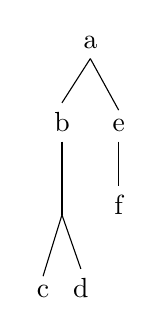
\begin{tikzpicture}
\Tree
[.a
[.b [c d ] ] 
[.e [.f ] ] 
]
\end{tikzpicture}
\end{center}
{\songti 如果已知中序遍历的栈的操作序列,就可唯一地确定一棵二叉树。请编程输出该二叉树的后序遍历序列。
提示:本题有多种解法,仔细分析二叉树非递归遍历过程中栈的操作规律与遍历序列的关系,可将二叉树构造出来。}
\subsubsection{基本要求}
\begin{description}
    \item[输入] 第一行一个整数n,表示二叉树的结点个数。\\
    接下来2n行,每行描述一个栈操作,格式为:push X 表示将结点X压入栈中,pop 表示从栈中弹出一个结点。\\
(X用一个字符表示)\\
对于20\%的数据,0<n<=10\\
对于40\%的数据,0<n<=20\\
对于100\%的数据,0<n<=83\\
    \item[输出] 一行,后序遍历序列。
\end{description}
\subsubsection{数据结构设计}
\begin{enumerate}
    \item node 结构体
    \begin{itemize}
        \item value: 存储节点的值(字符类型)。
        \item l: 指向左子节点的指针。
        \item r: 指向右子节点的指针。
        \item node(char x): 构造函数,用于初始化节点,设置节点的值为 x,并将左右子节点指针初始化为 NULL。
    \end{itemize}
    \item operation 数组:
    \begin{itemize}
        \item 用于存储操作序列,每个操作是一个字符串。操作可以是 push 或 pop。
    \end{itemize}
\end{enumerate}
\begin{tcblisting}{listing engine=minted,boxrule=0.1mm,
colback=blue!5!white,colframe=blue!75!black,
listing only,left=5mm,enhanced,sharp corners=all,
overlay={\begin{tcbclipinterior}\fill[red!20!blue!20!white] (frame.south west)
rectangle ([xshift=5mm]frame.north west);\end{tcbclipinterior}},
minted language=c++,
minted style=tango,
minted options={fontsize=\small,breaklines,autogobble,linenos,numbersep=3mm}}
// 定义二叉树节点结构体
struct node {
    char value;  // 节点值
    node* l;     // 左子节点指针
    node* r;     // 右子节点指针
    node(char x) : value(x), l(NULL), r(NULL) {}  // 构造函数
};
\end{tcblisting}
\subsubsection{功能说明}
\begin{tcblisting}{listing engine=minted,boxrule=0.1mm,
colback=blue!5!white,colframe=blue!75!black,
listing only,left=5mm,enhanced,sharp corners=all,
overlay={\begin{tcbclipinterior}\fill[red!20!blue!20!white] (frame.south west)
rectangle ([xshift=5mm]frame.north west);\end{tcbclipinterior}},
minted language=c++,
minted style=tango,
minted options={fontsize=\small,breaklines,autogobble,linenos,numbersep=3mm}}
// 根据操作序列构建二叉树
node* buildtree(int n, string* operation) {
    stack<node*> st;  // 辅助栈,用于构建树
    node* root = NULL;  // 根节点
    node* cr = NULL;  // 当前节点

    for (int i = 0; i < 2 * n; i++) {
        string op = operation[i];
        if (op[1] == 'u') {  // 如果是 push 操作
            char value = op[op.length()-1];  // 获取节点值
            node* newnode = new node(value);  // 创建新节点
            if (root == NULL)   // 如果根节点为空,设置根节点
                root = newnode;
            else {
                if (cr->l == NULL) // 如果当前节点的左子节点为空,设置左子节点
                    cr->l = newnode;
                else   // 否则设置右子节点
                    cr->r = newnode;
            }
            st.push(newnode);  // 将新节点压入栈中
            cr = newnode;  // 更新当前节点
        }
        else {  // 如果是 pop 操作
            if (!st.empty()) {
                cr = st.top();  // 弹出栈顶节点,更新当前节点
                st.pop();
            }
        }
    }
    return root;  // 返回根节点
}
\end{tcblisting}
\begin{tcblisting}{listing engine=minted,boxrule=0.1mm,
colback=blue!5!white,colframe=blue!75!black,
listing only,left=5mm,enhanced,sharp corners=all,
overlay={\begin{tcbclipinterior}\fill[red!20!blue!20!white] (frame.south west)
rectangle ([xshift=5mm]frame.north west);\end{tcbclipinterior}},
minted language=c++,
minted style=tango,
minted options={fontsize=\small,breaklines,autogobble,linenos,numbersep=3mm}}
// 后序遍历并输出树的节点值
void post_print(node* root) {
    if (root == NULL)
        return;
    post_print(root->l);  // 递归处理左子树
    post_print(root->r);  // 递归处理右子树
    cout << root->value;  // 输出当前节点的值
}
\end{tcblisting}
\subsubsection{调试分析}
\begin{itemize}
    \item 在用栈的进出模拟递归的时候,由于是后序建树,要注意取栈顶和出栈的顺序,要先取栈顶保留,再元素出栈,然后再以栈顶作为节点进行建树。
    \item 在main函数中的读取操作时,我首先用的是getline(cin,str),但是运行之后发现完全不能正常输出,于是经过VS2022自带的debug工具之后,发现getline并未从输入流中读取到东西进入operation,但是在其他题目里都没什么问题,可能是这题的输入数据有一些我不清楚的地方,所以就索性使用cin了,如果是push,再将后面的字母用strcat拼接起来。
\end{itemize}
\subsubsection{总结与体会}
\begin{enumerate}
    \item 栈的应用
    \begin{itemize}
        \item 栈在构建二叉树的过程中起到了关键作用。通过栈可以方便地管理当前处理的节点,以及回溯到上一层节点。
        \item 栈的使用使得代码逻辑清晰,易于理解和实现。
    \end{itemize}
    \item 递归的优雅
    \begin{itemize}
        \item 递归在后序遍历的实现中展现了其优雅和简洁。通过递归,可以轻松地遍历树的每个节点,并按后序顺序输出。
        \item 递归的实现方式使得代码结构清晰,易于维护和扩展。
    \end{itemize}
    \item 内存的管理
    \begin{itemize}
        \item 内存管理是编程中的一个重要问题。代码中使用了 delete[] 来释放根节点的内存,但这只是删除了根节点,并没有递归删除所有节点。
        \item 正确的做法是递归删除所有节点,或者使用智能指针来管理内存。内存管理不当可能导致内存泄漏或程序崩溃。
    \end{itemize}
\end{enumerate}
\subsection{二叉树的同构}
\subsubsection{问题描述}
{\songti 给定两棵树T1和T2。如果T1可以通过若干次左右孩子互换变成T2,则我们称两棵树是“同构”的。例如图1给出的两棵树就是同构的,因为我们把其中一棵树的结点a、b、e的左右孩子互换后,就得到另外一棵树。而图2就不是同构的。}
\begin{figure}[htbp]
    \centering
    \includegraphics[width=0.6\linewidth]{Screenshot 2024-10-24 210608.png}
    \label{fig:enter-label}
\end{figure}
{\songti 现给定两棵树,请你判断它们是否是同构的。并计算每棵树的深度。}
\subsubsection{基本要求}
\begin{description}
    \item[输入] 第一行是一个非负整数N1,表示第1棵树的结点数;\\
随后N行,依次对应二叉树的N个结点(假设结点从0到N−1编号),每行有三项,分别是1个英文大写字母、其左孩子结点的编号、右孩子结点的编号。如果孩子结点为空,则在相应位置上给出“-”。给出的数据间用一个空格分隔。\\
接着一行是一个非负整数N2,表示第2棵树的结点数;\\
随后N行同上描述一样,依次对应二叉树的N个结点。\\
对于20\%的数据,有0<N1=N2<=10\\
对于40\%的数据,有0<=N1=N2<=100\\
对于100\%的数据,有0<=N1,N2<=10100\\
注意:题目不保证每个结点中存储的字母是不同的。
    \item[输出] 共三行。\\
第一行,如果两棵树是同构的,输出“Yes”,否则输出“No”。\\
后面两行分别是两棵树的深度。\\
\end{description}
\subsubsection{数据结构设计}
\begin{tcblisting}{listing engine=minted,boxrule=0.1mm,
colback=blue!5!white,colframe=blue!75!black,
listing only,left=5mm,enhanced,sharp corners=all,
overlay={\begin{tcbclipinterior}\fill[red!20!blue!20!white] (frame.south west)
rectangle ([xshift=5mm]frame.north west);\end{tcbclipinterior}},
minted language=c++,
minted style=tango,
minted options={fontsize=\small,breaklines,autogobble,linenos,numbersep=3mm}}
const int MAXN = 10105; // 假设树的最大节点数为10105
struct Node {
    char val;
    int lchild, rchild;
    Node(char x = '\0', int l = -1, int r = -1) : val(x), lchild(l), rchild(r) {}
};
Node tree1[MAXN], tree2[MAXN];
int degree1[MAXN], degree2[MAXN];//引入度的概念
\end{tcblisting}

\subsubsection{功能说明}
{\songti 以下是本题的核心代码,包括递归检查是否同构、查找树的根节点等,本题的读取部分也比较重要,所以也会附上部分main函数中的代码。}
\begin{tcblisting}{listing engine=minted,boxrule=0.1mm,
colback=blue!5!white,colframe=blue!75!black,
listing only,left=5mm,enhanced,sharp corners=all,
overlay={\begin{tcbclipinterior}\fill[red!20!blue!20!white] (frame.south west)
rectangle ([xshift=5mm]frame.north west);\end{tcbclipinterior}},
minted language=c++,
minted style=tango,
minted options={fontsize=\small,breaklines,autogobble,linenos,numbersep=3mm}}
// 检查两棵树是否同构
bool check(const Node tree1[], int root1, const Node tree2[], int root2) {
    // 如果两个节点都是空节点,则认为是同构的
    if (root1 == -1 && root2 == -1) return true;
    // 如果其中一个节点是空节点,另一个不是,则不同构
    if (root1 == -1 || root2 == -1) return false;
    // 如果两个节点的值不同,则不同构
    if (tree1[root1].val != tree2[root2].val) return false;

    // 递归检查两种可能的同构情况:
    // 1. 左子树对应左子树,右子树对应右子树
    // 2. 左子树对应右子树,右子树对应左子树
    return (check(tree1, tree1[root1].lchild, tree2, tree2[root2].lchild) &&
            check(tree1, tree1[root1].rchild, tree2, tree2[root2].rchild)) ||
           (check(tree1, tree1[root1].lchild, tree2, tree2[root2].rchild) &&
            check(tree1, tree1[root1].rchild, tree2, tree2[root2].lchild));
}
// 查找树的根节点
int find_root(const int degree[], int n) {
    // 遍历所有节点,找到入度为0的节点,即为根节点
    for (int i = 0; i < n; ++i) {
        if (degree[i] == 0) return i;
    }
    // 如果没有找到入度为0的节点,返回-1
    return -1;
}
\end{tcblisting}



\begin{tcblisting}{listing engine=minted,boxrule=0.1mm,
colback=blue!5!white,colframe=blue!75!black,
listing only,left=5mm,enhanced,sharp corners=all,
overlay={\begin{tcbclipinterior}\fill[red!20!blue!20!white] (frame.south west)
rectangle ([xshift=5mm]frame.north west);\end{tcbclipinterior}},
minted language=c++,
minted style=tango,
minted options={fontsize=\small,breaklines,autogobble,linenos,numbersep=3mm}}
for (int i = 0; i < n1; ++i) {
        char val;
        string lchild, rchild;
        cin >> val >> lchild >> rchild;
        // 将节点信息存储到全局数组中
        tree1[i] = { val, lchild == "-" ? -1 : stoi(lchild), rchild == "-" ? -1 : stoi(rchild) };
        // 更新节点的入度信息
        if (tree1[i].lchild != -1) degree1[tree1[i].lchild]++;
        if (tree1[i].rchild != -1) degree1[tree1[i].rchild]++;
    }

    cin >> n2; // 输入第二棵树的节点数

    // 读取第二棵树的节点信息
    for (int i = 0; i < n2; ++i) {
        char val;
        string lchild, rchild;
        cin >> val >> lchild >> rchild;
        // 将节点信息存储到全局数组中
        tree2[i] = { val, lchild == "-" ? -1 : stoi(lchild), rchild == "-" ? -1 : stoi(rchild) };
        // 更新节点的入度信息
        if (tree2[i].lchild != -1) degree2[tree2[i].lchild]++;
        if (tree2[i].rchild != -1) degree2[tree2[i].rchild]++;
    }

\end{tcblisting}
{\songti 以上是main函数中读取部分的代码,要注意的是在读取value值时,需要用字符串储存,因为既有可能读到‘-’,也有可能读到真正的数字,都需要按字符来读取,在存value的时候用stoi函数转换就好了。}
\subsubsection{调试分析}
\begin{itemize}
    \item 这题困扰本人好长时间,提交后除了前两个测试,其他都是内存超限,让我很困惑,经过仔细研究后发现,原来是我在一开始的时候读取左右孩子是用char型读取的,在数据大的时候如果有2位及以上数字的情况就不会读取成功,后来改成string型来储存就好了。
\end{itemize}
\subsubsection{总结与体会}
{\songti 通过这段代码的学习,我深刻体会到了模块化设计的重要性。将复杂的问题拆分成多个小问题,并通过函数实现每个小问题的解决方案,能够使代码结构清晰、易于理解和维护。递归是一种自然的树结构遍历方式,能够有效地解决问题,但也带来了一定的时间和空间开销。\\
在实际开发中,我们需要根据具体的需求和场景,选择合适的数据结构和算法。对于树结构的处理,递归是一种常用的方法,但在树的规模较大时,需要考虑时间和空间的优化。通过哈希表等数据结构,可以减少递归调用的次数,提高程序的效率。\\
此外,输入数据的处理和验证也是程序设计中的重要环节。合理的输入格式设计能够提高程序的易用性,而输入数据的验证逻辑能够提高程序的健壮性。在实际开发中,我们需要充分考虑用户的使用场景,设计合理的输入格式和验证逻辑,确保程序的正确性和稳定性。\\
总之,这段代码展示了如何通过递归的方式判断两棵二叉树是否同构,并计算树的深度。通过学习和分析这段代码,我不仅掌握了树结构的处理方法,还深刻体会到了模块化设计、递归实现和输入处理的重要性。这些知识和经验将对我今后的编程实践产生积极的影响。}
\subsection{感染二叉树需要的总时间}
\subsubsection{问题描述}
{\songti 给你一棵二叉树的根节点 root ,二叉树中节点的值\textbf{互不相同} 。另给你一个整数 start 。在第 0 分钟,\textbf{感染}将会从值为 start 的节点开始爆发。
每分钟,如果节点满足以下全部条件,就会被感染:}
\begin{itemize}
    \item 节点此前还没有感染。
    \item 节点与一个已感染节点相邻。
\end{itemize}
{\songti 返回感染整棵树需要的分钟数。}
\begin{figure}[htbp]
    \centering
    \includegraphics[width=0.6\linewidth]{Screenshot 2024-10-25 141708.png}
\end{figure}
{\songti \\例如上图中 start = 3,输出:4\\
\textbf{解释:}节点按以下过程被感染: - 第 0 分钟:节点 3 - 第 1 分钟:节点 1、10、6 - 第 2 分钟:节点5 - 第 3 分钟:节点 4 - 第 4 分钟:节点 9 和 2 感染整棵树需要 4 分钟,所以返回 4 。}

\subsubsection{基本要求}
\begin{description}
    \item[输入] 第一行包含两个整数n和start\\
接下来包含n行,描述n个节点的左、右孩子编号\\
0号节点为根节点,0<=start<n\\
对于20\%的数据,1<=n<=10\\
对于40\%的数据,1<=n<=1000\\
对于100\%的数据,1<=n<=100000
    \item[输出] 一个整数,表示感染整棵二叉树所需要的时间。
\end{description}
\subsubsection{数据结构设计}
{\songti 使用静态数组来储存树的节点是很常用的方法在算法题中是很常见的}
\begin{tcblisting}{listing engine=minted,boxrule=0.1mm,
colback=blue!5!white,colframe=blue!75!black,
listing only,left=5mm,enhanced,sharp corners=all,
overlay={\begin{tcbclipinterior}\fill[red!20!blue!20!white] (frame.south west)
rectangle ([xshift=5mm]frame.north west);\end{tcbclipinterior}},
minted language=c++,
minted style=tango,
minted options={fontsize=\small,breaklines,autogobble,linenos,numbersep=3mm}}
const int N = 100005;
struct Node {
    int value;
    int l, r;
    int father;
} tree[N];
\end{tcblisting}
\subsubsection{功能说明}
\begin{tcblisting}{listing engine=minted,boxrule=0.1mm,
colback=blue!5!white,colframe=blue!75!black,
listing only,left=5mm,enhanced,sharp corners=all,
overlay={\begin{tcbclipinterior}\fill[red!20!blue!20!white] (frame.south west)
rectangle ([xshift=5mm]frame.north west);\end{tcbclipinterior}},
minted language=c++,
minted style=tango,
minted options={fontsize=\small,breaklines,autogobble,linenos,numbersep=3mm}}
void buildTree(int n) {
for (int i = 0; i < n; i++) {
    tree[i].value = i; //0默认为根节点直接储存
    cin >> tree[i].l >> tree[i].r;
    if (tree[i].l != -1)
       tree[tree[i].l].father = i;
    if (tree[i].r != -1)
       tree[tree[i].r].father = i;
}
\end{tcblisting}
{\songti 之后是使用广度优先搜素算法进行感染时间的计算,使用了stl容器的queue队列,和vector来储存某节点是否被感染。使用queue是因为,我觉得已经过了手写基本数据结构的阶段了,毕竟有关队列的作业确实是手动维护的队列,到了这里就没必要硬性要求手动了,毕竟这次作业的核心是树,而不是队列,队列只是工具,而简便的stl容器更能清晰的体现树的使用。而此处使用的vector也没有使用vector的更多高级用法,其实就相当于用了一个new。}
\begin{tcblisting}{listing engine=minted,boxrule=0.1mm,
colback=blue!5!white,colframe=blue!75!black,
listing only,left=5mm,enhanced,sharp corners=all,
overlay={\begin{tcbclipinterior}\fill[red!20!blue!20!white] (frame.south west)
rectangle ([xshift=5mm]frame.north west);\end{tcbclipinterior}},
minted language=c++,
minted style=tango,
minted options={fontsize=\small,breaklines,autogobble,linenos,numbersep=3mm}}
int bfs(int start, int n) {  //bfs就是队列
    queue<int> q;
    vector<bool> infected(n, false);
    q.push(start);  //先让感染源进队
    infected[start] = true; 
    int time = 0;
    while (!q.empty()) {
        int size = q.size(); //很好地控制了循环的次数,保证对队列中的每个元素进行一次操作
        for (int i = 0; i < size; ++i) {
            int node = q.front();  //很经典的bfs队列使用
            q.pop();
            if (tree[node].l != -1 && !infected[tree[node].l]) {
                infected[tree[node].l] = true;
                q.push(tree[node].l);
            }
            if (tree[node].r != -1 && !infected[tree[node].r]) {
                infected[tree[node].r] = true;
                q.push(tree[node].r);
            }
            if (tree[node].father != -1 && !infected[tree[node].father]) {
                infected[tree[node].father] = true;
                q.push(tree[node].father);
            }
        }
        if (!q.empty()) {  //感染一圈后,更新time
            time++;
        }
    }
    return time;
}
\end{tcblisting}

\subsubsection{调试分析}
\begin{itemize}
    \item 本人一开始想用深度优先搜索尝试,但是计算的结果不对,而且确实也不是太适合解决这个问题,于是就换成bfs。我总结到还是我对bfs、dfs这两种算法理解不到位,应该可以很明确的分辨出来这题确实适合用bfs,以一点为中心扩散,是很形象的广度优先思维。
\end{itemize}

\subsubsection{总结与体会}
\begin{description}
    \item[广度优先搜索的应用] BFS 是一种非常适合用于层级遍历和最短路径问题的算法。在这个问题中,BFS 能够有效地模拟病毒传播的过程,并且能够准确地计算出传播到整个树所需的时间。BFS 的层级遍历特性使得每一层的节点都能在同一时间步内被处理,从而保证了时间的准确性。
    \item[复杂度分析] 构建树的时间复杂度为 O(n),其中 n 是节点数量。\\
BFS 的时间复杂度为 O(n),因为每个节点最多被访问一次。\\
整体时间复杂度为 O(n),适用于中等规模的树结构。
\end{description}
\subsection{树的重构}
\subsubsection{问题描述}
{\songti 树木在计算机科学中有许多应用。 也许最常用的树是二叉树,但也有其他的同样有用的树类型。 其中一个例子是有序树(任意节点的子树是有序的)。 每个节点的子节点数是可变的,并且数量没有限制。 一般而言, 有序树由有限节点集合T组成,并且满足:}
\begin{enumerate}
    \item 其中一个节点置为根节点,定义为root(T);
    \item 其他节点被划分为若干子集T1,T2,...Tm,每个子集都是一个树.
\end{enumerate}
{\songti 同样定义root(T1),root(T2),...root(Tm)为root(T)的孩子,其中root(Ti)是第i个孩子。节点root(T1),...root(Tm)是兄弟节点。通常将一个有序树表示为二叉树是更加有用的,这样每个节点可以存储在相同内存空间中。有序树到二叉树的转化步骤为:}
\begin{enumerate}
    \item 去除每个节点与其子节点的边
    \item 对于每一个节点,在它与第一个孩子节点(如果存在)之间添加一条边,作为该节点的左孩子
    \item 对于每一个节点,在它与下一个兄弟节点(如果存在)之间添加一条边,作为该节点的右孩子
\end{enumerate}
\begin{figure}[htbp]
    \centering
    \includegraphics[width=0.4\linewidth]{Screenshot 2024-10-27 105702.png}
\end{figure}
{\songti 在大多数情况下,树的深度(从根节点到叶子节点的边数的最大值)都会在转化后增加。这是不希望发生的事情因为很多算法的复杂度都取决于树的深度。\\
现在,需要你实现一个程序来计算转化前后的树的深度。}
\subsubsection{基本要求}
\begin{description}
    \item[输入] 输入由多行组成,每一行都是一棵树的深度优先遍历时的方向。其中d表示下行(down),u表示上行(up)。\\
例如上面的树就是dudduduudu,表示从0下行到1,1上行到0,0下行到2等等。输入的截止为以\#开始的行。\\
可以假设每棵树至少含有2个节点,最多10000个节点。
    \item[输出] 对每棵树,打印转化前后的树的深度,采用以下格式 Tree t: h1 => h2。其中t表示样例编号(从1开始),h1是转化前的树的深度,h2是转化后的树的深度。
\end{description}
\subsubsection{数据结构设计}
\begin{tcblisting}{listing engine=minted,boxrule=0.1mm,
colback=blue!5!white,colframe=blue!75!black,
listing only,left=5mm,enhanced,sharp corners=all,
overlay={\begin{tcbclipinterior}\fill[red!20!blue!20!white] (frame.south west)
rectangle ([xshift=5mm]frame.north west);\end{tcbclipinterior}},
minted language=c++,
minted style=tango,
minted options={fontsize=\small,breaklines,autogobble,linenos,numbersep=3mm}}
const int N = 10005;
struct onode { //储存原多叉树的节点
    vector<int>child; //用vector来存孩子(其实和new没什么区别)
    int next=-1; //表示右侧兄弟节点
}otree[N];
struct bnode {
    int l, r;
}btree[N];
\end{tcblisting}
\subsubsection{功能说明}
\begin{tcblisting}{listing engine=minted,boxrule=0.1mm,
colback=blue!5!white,colframe=blue!75!black,
listing only,left=5mm,enhanced,sharp corners=all,
overlay={\begin{tcbclipinterior}\fill[red!20!blue!20!white] (frame.south west)
rectangle ([xshift=5mm]frame.north west);\end{tcbclipinterior}},
minted language=c++,
minted style=tango,
minted options={fontsize=\small,breaklines,autogobble,linenos,numbersep=3mm}}
void buildbtree() {  // 建二叉树
    for (int i = 0; i <= n; i++) {
        if (!otree[i].child.empty())
            btree[i].l = otree[i].child[0];
        if (otree[i].next != -1)
            btree[i].r = otree[i].next;
    }
}
\end{tcblisting}
\begin{tcblisting}{listing engine=minted,boxrule=0.1mm,
colback=blue!5!white,colframe=blue!75!black,
listing only,left=5mm,enhanced,sharp corners=all,
overlay={\begin{tcbclipinterior}\fill[red!20!blue!20!white] (frame.south west)
rectangle ([xshift=5mm]frame.north west);\end{tcbclipinterior}},
minted language=c++,
minted style=tango,
minted options={fontsize=\small,breaklines,autogobble,linenos,numbersep=3mm}}
int n; //n为总节点数
void buildotree(string s) {  // 建初始树
    stack<int> st;
    st.push(0);  //0节点默认为根节点进栈
    for (int i = 0; i < int(s.size()); i++) {
        if (s[i] == 'd') {
            n++;  //读到d则新增节点
            otree[st.top()].child.push_back(n); //此为栈顶节点的孩子
            st.push(n);
        }
        else if (s[i] == 'u') {
            int x = st.top();
            st.pop();
            if (i + 1 < int(s.size()) && s[i + 1] == 'd') {
                otree[x].next = n + 1;
            }
        }
    }
}
\end{tcblisting}
{\songti 计算树的深度的代码就不赘述了,基本是有固定的模式。}
\subsubsection{调试分析}
\begin{itemize}
    \item 在测试题目界面的样例时,总发现每一串du下会输出两行Tree x=>y,第一行的值还是有意义的,但是第二行都是0了,一开始还认为是我的代码逻辑有问题,检查后才发现是,oj界面给的测试样例输入多了一行空行,导致我的getline多读了一行空行,所以才有一行Tree 0=>0,提交后发现内部测试其实是没有空行的...
    \item 计算树深的代码要根据题目要求做一些微调,可能具体题目的一些具体要求不同。
\end{itemize}
\subsubsection{总结与体会}
\begin{description}
    \item[选用栈的数据结构来模拟递归] 使用栈来构建树是一种非常有效的方法,特别是在处理嵌套结构时。栈能够帮助我们轻松地管理节点的添加和回溯。将多叉树转换为二叉树时,需要仔细考虑如何映射节点的关系,特别是左子节点和右子节点的选择。
\end{description}
\subsection{最近公共祖先}
\subsubsection{问题描述}
{\songti 给出一颗多叉树,请你求出两个节点的最近公共祖先。
一个节点的祖先节点可以是该节点本身,树中任意两个节点都至少有一个共同祖先,即根节点。}
\subsubsection{基本要求}
\begin{description}
    \item[输入] 输入数据包含T个测试样本,每个样本i包含Ni个节点和Ni-1条边和Mi个问题,树中节点从1到Ni编号\\
输入第一行是测试样本数T\\
每个测试样本i第一行为两个整数Ni和Mi\\
接下来Ni-1行,每行2个整数a、b,表示a是b的父节点\\
接下来Mi行,每行两个整数x、y,表示询问x和y的共同祖先\\
对于100\%的数据,\\
1<=T<=100;\\
5<=N<=1000;\\
5<=M<=1000;
    \item[输出] 对于每一个询问输出一个整数,表示共同祖先的编号
\end{description}
\subsubsection{数据结构设计}
\begin{tcblisting}{listing engine=minted,boxrule=0.1mm,
colback=blue!5!white,colframe=blue!75!black,
listing only,left=5mm,enhanced,sharp corners=all,
overlay={\begin{tcbclipinterior}\fill[red!20!blue!20!white] (frame.south west)
rectangle ([xshift=5mm]frame.north west);\end{tcbclipinterior}},
minted language=c++,
minted style=tango,
minted options={fontsize=\small,breaklines,autogobble,linenos,numbersep=3mm}}
// 定义边的结构体
struct Edge {
    int to, next;  // to: 边的终点,next: 下一条边的索引
} e[2010];
// 全局变量
int head[1010], tot;  // head: 存储每个节点的第一条边的索引,tot: 边的总数
int depth[1010], fa[1010][11], lg[1010];  // depth: 存储每个节点的深度,fa: 存储每个节点的第 2^i 个祖先,lg: 存储每个数的对数(以2为底)
bool is_root[1010];  // 用于标记哪个节点是根节点
\end{tcblisting}
{\songti 本题采用了链式向前星建图法,而且由于是无向图,且该建图法存的是边,所以结构体数组总量要大概开2倍。}
\subsubsection{功能说明}
\begin{tcblisting}{listing engine=minted,boxrule=0.1mm,
colback=blue!5!white,colframe=blue!75!black,
listing only,left=5mm,enhanced,sharp corners=all,
overlay={\begin{tcbclipinterior}\fill[red!20!blue!20!white] (frame.south west)
rectangle ([xshift=5mm]frame.north west);\end{tcbclipinterior}},
minted language=c++,
minted style=tango,
minted options={fontsize=\small,breaklines,autogobble,linenos,numbersep=3mm}}
// 添加边
void add(int x, int y) {
    e[++tot].to = y;  // 边的终点
    e[tot].next = head[x];  // 下一条边的索引
    head[x] = tot;  // 更新节点的第一条边的索引
}
// 初始化对数表
void init_lg(int n) {
    lg[1] = 0;  // log2(1) = 0
    for (int i = 2; i <= n; i++) 
        lg[i] = lg[i >> 1] + 1;  // log2(i) = log2(i/2) + 1
}
\end{tcblisting}

\begin{tcblisting}{listing engine=minted,boxrule=0.1mm,
colback=blue!5!white,colframe=blue!75!black,
listing only,left=5mm,enhanced,sharp corners=all,
overlay={\begin{tcbclipinterior}\fill[red!20!blue!20!white] (frame.south west)
rectangle ([xshift=5mm]frame.north west);\end{tcbclipinterior}},
minted language=c++,
minted style=tango,
minted options={fontsize=\small,breaklines,autogobble,linenos,numbersep=3mm}}
// 深度优先搜索(DFS)
void dfs(int now, int father) {
    fa[now][0] = father;  // 记录当前节点的父节点
    depth[now] = depth[father] + 1;  // 计算当前节点的深度
    // 预处理每个节点的第 2^i 个祖先
    for (int i = 1; (1 << i) <= depth[now]; i++) {
        fa[now][i] = fa[fa[now][i - 1]][i - 1];  // 倍增法
    }//意思是now的2^i祖先等于now的2^(i-1)祖先的2^(i-1)祖先
    /2^i = 2^(i-1) + 2^(i-1)
    // 遍历当前节点的所有子节点
    for (int i = head[now]; i; i = e[i].next) {
        int to = e[i].to;  // 子节点
        if (to != father)   // 避免重复访问父节点
            dfs(to, now);  // 递归处理子节点
    }
}
// 计算最近公共祖先(LCA)
int LCA(int x, int y) {
    if (depth[x] < depth[y]) swap(x, y);  // 确保 x 的深度不小于 y

    // 将 x 跳到与 y 同一深度
    for (int i = lg[depth[x]]; i >= 0; i--) {
        if (depth[x] - (1 << i) >= depth[y]) 
            x = fa[x][i];  // 跳到第 2^i 个祖先
    }
    if (x == y) return x;  // 如果 x 和 y 已经相同,直接返回
    // 同时向上跳,直到找到 LCA
    for (int i = lg[depth[x]]; i >= 0; i--) {
        if (fa[x][i] != fa[y][i]) {  // 如果第 2^i 个祖先不同
            x = fa[x][i];  // 跳到第 2^i 个祖先
            y = fa[y][i];  // 跳到第 2^i 个祖先
        }
    }
    return fa[x][0];  // 返回 x 的父节点,即 LCA
}
\end{tcblisting}

\begin{tcblisting}{listing engine=minted,boxrule=0.1mm,
colback=blue!5!white,colframe=blue!75!black,
listing only,left=5mm,enhanced,sharp corners=all,
overlay={\begin{tcbclipinterior}\fill[red!20!blue!20!white] (frame.south west)
rectangle ([xshift=5mm]frame.north west);\end{tcbclipinterior}},
minted language=c++,
minted style=tango,
minted options={fontsize=\small,breaklines,autogobble,linenos,numbersep=3mm}}
// 找到根节点
int find_root(int n) {
    for (int i = 1; i <= n; i++) {
        if (is_root[i]) return i;  // 找到第一个标记为根的节点
    }
    return 1;  // 不应该到达这里
}
\end{tcblisting}
\subsubsection{调试分析}
{\songti 其实是本人之前做过洛谷求最近公共祖先的模板题,使用倍增算法进行了常数优化,并且优化了一下代码结构,就形成了这道题的代码。}
\subsubsection{总结与体会}
\begin{description}
    \item[\textbf{链式向前星}] 链式向前星是一种高效的图存储结构,特别适用于稀疏图。它的核心思想是通过链表的方式存储每个节点的邻接边,从而节省空间。链式向前星的主要优势在于:
    \begin{enumerate}[label=\arabic*.]
        \item \textbf{节省空间}:相比于邻接矩阵,链式向前星只存储实际存在的边,避免了稀疏图中的大量无效空间占用。
        \item \textbf{高效遍历}:通过 head 和 next 指针,可以高效地遍历每个节点的邻接边,时间复杂度为 \(O(E)\),其中 \(E\) 是边的数量。
    \end{enumerate}
    在代码中,链式向前星通过一个数组 head 存储每个节点的第一条边的索引,并通过 next 指针将所有与该节点相连的边串联起来。这种结构使得图的存储和遍历变得非常高效。
    
    \item[\textbf{倍增算法求解LCA}] 倍增算法是一种用于快速求解最近公共祖先(LCA)的算法。它通过预处理每个节点的第 \(2^i\) 个祖先,从而在查询时能够快速跳转到目标节点。倍增算法的主要优势在于:
    \begin{enumerate}[label=\arabic*.]
        \item \textbf{预处理时间复杂度}:预处理的时间复杂度为 \(O(n \log n)\),适用于大规模树结构的预处理。
        \item \textbf{查询时间复杂度}:每次查询的时间复杂度为 \(O(\log n)\),适用于多次查询的场景。
    \end{enumerate}
    在代码中,倍增算法通过深度优先搜索(DFS)预处理每个节点的深度和第 \(2^i\) 个祖先。预处理完成后,查询 LCA 时可以通过二分查找的方式快速跳转到目标节点,从而实现高效的 LCA 查询。
\end{description}
\subsection{求树的后序}
\subsubsection{问题描述}
{\songti 给出二叉树的前序遍历和中序遍历,求树的后序遍历}
\subsubsection{基本要求}
\begin{description}
    \item[输入] 输入包含若干行,每一行有两个字符串,中间用空格隔开\\
同行的两个字符串从左到右分别表示树的前序遍历和中序遍历,由单个字符组成,每个字符表示一个节点\\
字符仅包括大小写英文字母和数字,最多62个\\
输入保证一颗二叉树内不存在相同的节点
    \item[输出] 每一行输入对应一行输出\\
若给出的前序遍历和中序遍历对应存在一棵二叉树,则输出其后序遍历\\
否则输出Error
\end{description}
\subsubsection{数据结构设计}
{\songti 本题倒没有什么复杂的数据结构,只是先定义两个字符串,分别来储存中序和前序,在后续的功能说明部分详细展示递归求后续的关键代码。}
\begin{tcblisting}{listing engine=minted,boxrule=0.1mm,
colback=blue!5!white,colframe=blue!75!black,
listing only,left=5mm,enhanced,sharp corners=all,
overlay={\begin{tcbclipinterior}\fill[red!20!blue!20!white] (frame.south west)
rectangle ([xshift=5mm]frame.north west);\end{tcbclipinterior}},
minted language=c++,
minted style=tango,
minted options={fontsize=\small,breaklines,autogobble,linenos,numbersep=3mm}}
string inorder, preorder;
\end{tcblisting}
\subsubsection{功能说明}
\begin{tcblisting}{listing engine=minted,boxrule=0.1mm,
colback=blue!5!white,colframe=blue!75!black,
listing only,left=5mm,enhanced,sharp corners=all,
overlay={\begin{tcbclipinterior}\fill[red!20!blue!20!white] (frame.south west)
rectangle ([xshift=5mm]frame.north west);\end{tcbclipinterior}},
minted language=c++,
minted style=tango,
minted options={fontsize=\small,breaklines,autogobble,linenos,numbersep=3mm}}
int error_or_not;// 全局变量,用于标记是否出现错误
// 判断给定的先序遍历和中序遍历是否能构成一棵合法的二叉树
void judge(string in, string pre)
{
    if (in.size() == 0) 
        return;// 如果中序遍历或先序遍历为空,直接返回
    // 如果中序遍历和先序遍历都只有一个节点,但节点值不同,则说明输入错误
    else if (in.size() == 1 && pre.size() == 1 && in != pre) {
        error_or_not = 1;
        return;
    }
    char root = pre[0];// 先序遍历的第一个节点是根节点
    int m = in.find(root);// 在中序遍历中找到根节点的位置
    string insubls = in.substr(0, m); // 左子树的中序遍历
    string insubrs = in.substr(m + 1); // 右子树的中序遍历
    string presubls = pre.substr(1, m); // 左子树的先序遍历
    string presubrs = pre.substr(m + 1); // 右子树的先序遍历
    // 如果左子树或右子树的节点数不匹配,说明输入错误
    if (insubls.size() != presubls.size() || insubrs.size() != presubrs.size()) {
        error_or_not = 1;
        return;
    }
    judge(insubls, presubls); // 递归判断左子树
    judge(insubrs, presubrs); // 递归判断右子树
}
\end{tcblisting}

\begin{tcblisting}{listing engine=minted,boxrule=0.1mm,
colback=blue!5!white,colframe=blue!75!black,
listing only,left=5mm,enhanced,sharp corners=all,
overlay={\begin{tcbclipinterior}\fill[red!20!blue!20!white] (frame.south west)
rectangle ([xshift=5mm]frame.north west);\end{tcbclipinterior}},
minted language=c++,
minted style=tango,
minted options={fontsize=\small,breaklines,autogobble,linenos,numbersep=3mm}}
// 根据中序遍历和先序遍历输出后序遍历
void find_postorder(string in, string pre) {
    if (in.size() == 0) 
        return;// 如果中序遍历为空,直接返回
    char root = pre[0]; // 先序遍历的第一个节点是根节点
    int m = in.find(root);// 在中序遍历中找到根节点的位置
    string insubls = in.substr(0, m); // 左子树的中序遍历
    string insubrs = in.substr(m + 1); // 右子树的中序遍历
    string presubls = pre.substr(1, m); // 左子树的先序遍历
    string presubrs = pre.substr(m + 1); // 右子树的先序遍历
    
    find_postorder(insubls, presubls);// 递归处理左子树的后序遍历
    find_postorder(insubrs, presubrs);// 递归处理右子树的后序遍历
    // 后序遍历最后输出根节点
    cout << root;
}
\end{tcblisting}
{\songti 本题很关键的一环就是判断题目输入的前序和中序是否可以表示同一棵二叉树,不能的话直接输出ERROR并退出,而该功能是由judge函数实现的,先全局定义一个error\_or\_not的变量,通过改变和读取该变量的值,可以在main函数中做出准确的输出。}
\subsubsection{调试分析}
{\songti 初期的想法是想在生成后序遍历序列的函数里判断是否error的,但是后来发现这样划分函数不方便效果也不太好,于是就单独提炼出一个judge函数来判断。\\
而是否error的判断条件就是,首先要满足给出的先序序列和中序序列的长度是一样的,其次要满足每次递归的左右子树是相同且合理的。}

\subsubsection{总结与体会}
{\songti 完成本题后,我深刻体会到了为什么已知中序前序可以求后序或者已知中序后序可以求前序,而不能已知前序后序来求中序,而对其的错误的判断也在几次调试之后理解掌握的更全面。更深刻地理解了二叉树这一数据结构。}

\subsection{表达式树}
\subsubsection{问题描述}
{\songti 任何一个表达式,都可以用一棵表达式树来表示。例如,表达式a+b*c,可以表示为如下的表达式树:\\}
\begin{center}
\begin{tikzpicture}
\Tree
[.+
[.a  ] 
[.* [b c ] ] 
]
\end{tikzpicture}
\end{center}
{\songti 现在,给你一个中缀表达式,这个中缀表达式用变量来表示(不含数字),请你将这个中缀表达式用表达式二叉树的形式输出出来。}
\subsubsection{基本要求}
\begin{description}
    \item[输入格式] 输入分为三个部分。\\
第一部分为一行,即中缀表达式(长度不大于50)。\\
中缀表达式可能含有小写字母代表变量(a-z),也可能含有运算符(+、-、*、/、小括号),\\
不含有数字,也不含有空格。\\
第二部分为一个整数n(n <= 10),表示中缀表达式的变量数。\\
第三部分有n行,每行格式为C x,C为变量的字符,x为该变量的值。\\
对于20\%的数据,1<=n<=3,1<=x<=5;\\
对于40\%的数据,1<=n<=5,1<=x<=10;\\
对于100\%的数据,1<=n<=10,1<=x<=100;
    \item[输出格式] 输出分为三个部分,第一个部分为该表达式的逆波兰式,即该表达式树的后根遍历结果。占一行。\\
第二部分为表达式树的显示,如样例输出所示。\\
如果该二叉树是一棵满二叉树,则最底部的叶子结点,分别占据横坐标的第1、3、5、7……个位置(最左边的坐标是1),
然后它们的父结点的横坐标,在两个子结点的中间。\\
如果不是满二叉树,则没有结点的地方,用空格填充(但请略去所有的行末空格)。\\
每一行父结点与子结点中隔开一行,用斜杠(/)与反斜杠($\backslash$)来表示树的关系。\\
/出现的横坐标位置为父结点的横坐标偏左一格,$\backslash$出现的横坐标位置为父结点的横坐标偏右一格。\\
也就是说,如果树高为m,则输出就有2m-1行。\\
第三部分为一个整数,表示将值代入变量之后,该中缀表达式的值。需要注意的一点是,除法代表整除运算,即舍弃小数点后的部分。\\
同时,测试数据保证不会出现除以0的现象。
\end{description}
\subsubsection{数据结构设计}
\begin{tcblisting}{listing engine=minted,boxrule=0.1mm,
colback=blue!5!white,colframe=blue!75!black,
listing only,left=5mm,enhanced,sharp corners=all,
overlay={\begin{tcbclipinterior}\fill[red!20!blue!20!white] (frame.south west)
rectangle ([xshift=5mm]frame.north west);\end{tcbclipinterior}},
minted language=c++,
minted style=tango,
minted options={fontsize=\small,breaklines,autogobble,linenos,numbersep=3mm}}
struct TreeNode {// 定义树节点结构体
    char value; // 节点值
    int height; // 节点高度
    TreeNode* left; // 左子节点
    TreeNode* right; // 右子节点
    TreeNode(char val) : value(val), height(1), left(nullptr), right(nullptr) {} // 构造函数
};
\end{tcblisting}
\subsubsection{功能说明}
\begin{tcblisting}{listing engine=minted,boxrule=0.1mm,
colback=blue!5!white,colframe=blue!75!black,
listing only,left=5mm,enhanced,sharp corners=all,
overlay={\begin{tcbclipinterior}\fill[red!20!blue!20!white] (frame.south west)
rectangle ([xshift=5mm]frame.north west);\end{tcbclipinterior}},
minted language=c++,
minted style=tango,
minted options={fontsize=\small,breaklines,autogobble,linenos,numbersep=3mm}}
int precedence(char op) {  // 获取操作符优先级
    if (op == '+' || op == '-') return 1; // 加减优先级为1
    if (op == '*' || op == '/') return 2; // 乘除优先级为2
    return 0; // 其他字符优先级为0
}
// 应用操作符,构建表达式树
void apply_operator(TreeNode** nodes, int& node_top, char* operators, int& op_top) {
    char op = operators[op_top--];//弹出操作符栈顶元素
    TreeNode* right = nodes[node_top--];//弹出节点栈顶元素作为右子节点
    TreeNode* left = nodes[node_top--];//弹出节点栈顶元素作为左子节点
    TreeNode* newNode = new TreeNode(op); // 创建新节点
    newNode->left = left; // 设置左子节点
    newNode->right = right; // 设置右子节点
    newNode->height = max(left->height, right->height) + 1; // 计算新
    nodes[++node_top] = newNode; // 将新节点压入节点栈      //节点高度
}
\end{tcblisting}

\begin{tcblisting}{listing engine=minted,boxrule=0.1mm,
colback=blue!5!white,colframe=blue!75!black,
listing only,left=5mm,enhanced,sharp corners=all,
overlay={\begin{tcbclipinterior}\fill[red!20!blue!20!white] (frame.south west)
rectangle ([xshift=5mm]frame.north west);\end{tcbclipinterior}},
minted language=c++,
minted style=tango,
minted options={fontsize=\small,breaklines,autogobble,linenos,numbersep=3mm}}
// 构建表达式树
TreeNode* build_expression_tree(const char* expression) {
    TreeNode* nodes[100]; // 节点栈
    char operators[100]; // 操作符栈
    int node_top = -1, op_top = -1; // 栈顶指针初始化为-1
    for (int i = 0; expression[i]; ++i) {
        char ch = expression[i];
        if (isalpha(ch)) { // 如果是字母(变量)
            nodes[++node_top] = new TreeNode(ch); // 创建新节点并压入节点栈
        }
        else if (ch == '(') { // 如果是左括号
            operators[++op_top] = ch; // 压入操作符栈
        }
        else if (ch == ')') { // 如果是右括号
            while (op_top >= 0 && operators[op_top] != '(') { // 弹出操作符栈中的操作符直到遇到左括号
                apply_operator(nodes, node_top, operators, op_top);
            }
            --op_top; // 弹出左括号
        }
        else { // 如果是操作符
            while (op_top >= 0 && precedence(operators[op_top]) >= precedence(ch)) { // 弹出优先级高的操作符
                apply_operator(nodes, node_top, operators, op_top);
            }
            operators[++op_top] = ch; // 将当前操作符压入操作符栈
        }
    }
    while (op_top >= 0) { // 处理剩余的操作符
        apply_operator(nodes, node_top, operators, op_top);
    }
    return nodes[0]; // 返回根节点
}
\end{tcblisting}
\begin{tcblisting}{listing engine=minted,boxrule=0.1mm,
colback=blue!5!white,colframe=blue!75!black,
listing only,left=5mm,enhanced,sharp corners=all,
overlay={\begin{tcbclipinterior}\fill[red!20!blue!20!white] (frame.south west)
rectangle ([xshift=5mm]frame.north west);\end{tcbclipinterior}},
minted language=c++,
minted style=tango,
minted options={fontsize=\small,breaklines,autogobble,linenos,numbersep=3mm}}
// 后序遍历表达式树,生成后缀表达式
void postorder_traversal(TreeNode* root, char* result, int& index) {
    if (root == nullptr) return;
    postorder_traversal(root->left, result, index); // 遍历左子树
    postorder_traversal(root->right, result, index); // 遍历右子树
    result[index++] = root->value; // 将节点值加入结果数组
}

// 计算表达式的值
int calculate_expression(TreeNode* root, const int* values) {
    if (root == nullptr) return 0;
    if (isalpha(root->value)) { // 如果是变量
        return values[root->value - 'a']; // 返回变量对应的值
    }

    int left_val = calculate_expression(root->left, values); // 计算左子树的值
    int right_val = calculate_expression(root->right, values); // 计算右子树的值

    if (root->value == '+') return left_val + right_val; // 加法
    if (root->value == '-') return left_val - right_val; // 减法
    if (root->value == '*') return left_val * right_val; // 乘法
    if (root->value == '/') return left_val / right_val; // 除法

    return 0;
}
\end{tcblisting}
\begin{tcblisting}{listing engine=minted,boxrule=0.1mm,
colback=blue!5!white,colframe=blue!75!black,
listing only,left=5mm,enhanced,sharp corners=all,
overlay={\begin{tcbclipinterior}\fill[red!20!blue!20!white] (frame.south west)
rectangle ([xshift=5mm]frame.north west);\end{tcbclipinterior}},
minted language=c++,
minted style=tango,
minted options={fontsize=\small,breaklines,autogobble,linenos,numbersep=3mm}}
// 打印树结构
void print_tree(TreeNode* root, int level, int pos, char** lines, int& max_level) {
    if (root == nullptr) return;

    // 确保 lines 数组有足够的行数
    if (level > max_level) max_level = level;

    // 确保当前行的长度足够
    while (strlen(lines[level]) < pos) {
        strcat(lines[level], " ");
    }

    // 添加当前节点的值
    char temp[2];
    temp[0] = root->value;
    temp[1] = '\0';
    strcat(lines[level], temp);

    // 递归打印左子树和右子树
    if (root->left) {
        // 添加左子树的连接线
        if (level + 1 > max_level) max_level = level + 1;
        while (strlen(lines[level + 1]) < pos - 1) {
            strcat(lines[level + 1], " ");
        }
        strcat(lines[level + 1], "/");

        // 递归打印左子树
        print_tree(root->left, level + 2, pos - (1 << (root->height - 2)), lines, max_level);
    }
\end{tcblisting}
\begin{tcblisting}{listing engine=minted,boxrule=0.1mm,
colback=blue!5!white,colframe=blue!75!black,
listing only,left=5mm,enhanced,sharp corners=all,
overlay={\begin{tcbclipinterior}\fill[red!20!blue!20!white] (frame.south west)
rectangle ([xshift=5mm]frame.north west);\end{tcbclipinterior}},
minted language=c++,
minted style=tango,
minted options={fontsize=\small,breaklines,autogobble,linenos,numbersep=3mm}}
if (root->right) {
        // 添加右子树的连接线
        if (level + 1 > max_level) max_level = level + 1;
        while (strlen(lines[level + 1]) < pos + 1) {
            strcat(lines[level + 1], " ");
        }
        strcat(lines[level + 1], "\\");

        // 递归打印右子树
        print_tree(root->right, level + 2, pos + (1 << (root->height - 2)), lines, max_level);
    }
}
\end{tcblisting}

\subsubsection{调试分析}
{\songti 在打印树结构时,发现某些节点的位置不正确,导致树结构显示混乱。于是我选择在 print\_tree 函数中添加调试输出,打印每个节点的位置信息,确保节点的位置计算正确。
通过这样打印中间变量的方法,我才发现某些节点的位置计算不正确,导致树结构显示错误。
那么解决方案就是1调整 print\_tree 函数中的位置计算逻辑,确保每个节点的位置计算正确。同时,优化树结构的打印逻辑,确保树结构显示清晰。}
\subsubsection{总结与体会}
\begin{itemize}
    \item 表达式树的构建和遍历涉及到复杂的逻辑,需要仔细处理操作符的优先级、节点的遍历顺序和计算逻辑。在调试过程中,我们发现代码的逻辑复杂性较高,容易出现错误。因此,在编写代码时,需要仔细设计算法,确保逻辑的正确性。
    \item 在调试过程中,我们使用了调试输出、断点调试等工具,帮助我们快速定位问题。调试工具的使用对于解决复杂问题非常重要,能够提高调试效率。
    \item 在调试过程中,我们发现测试对于验证代码的正确性非常重要。通过编写测试用例,我们能够快速验证代码的正确性,发现潜在的问题。因此,在编写代码时,需要编写充分的测试用例,确保代码的正确性。
\end{itemize}
\subsection{实验总结}
{\songti 通过本次实验,我们深入探索了二叉树的多种算法,包括非递归遍历、同构判断、树的重构、感染时间计算、最近公共祖先查找、表达式树构建与计算以及后序遍历的求解。这些实验不仅加深了我们对二叉树结构及其操作的理解,还让我们认识到算法设计的灵活性和性能分析的重要性。在实际应用中,二叉树算法广泛应用于数据处理、编译器设计、网络传播等多个领域,展示了其强大的实用价值。通过调试和测试,我们学会了如何快速定位和解决问题,同时也体会到团队合作和知识共享在解决复杂问题中的关键作用。总的来说,本次实验不仅提升了我们的算法设计和实现能力,还为我们未来的学习和工作中提供了宝贵的经验和启示。}

\end{document}
